\subsection{Changes to accessibility settings}
A customer request was made to create a feature which could add a pictogram to specific users in the system. 
Previously, we have the option of assigning the pictogram to the user, as private, or available to everyone, as public.

We change the public to be institution wide, meaning the pictogram is available to all the guardians and citizens of the institution.
The private option is changed to be available for specific citizens, chosen from a list which contains the citizens assigned to the currently logged in guardian.
To avoid confusion, it is decided that the button to add citizens and the list with the citizens is hidden until the user checks the citizen radio button.

This change require a significant overhaul in the GUI of the save dialogue, the resulting GUI can be seen in \figref{fig:save_dialogue2}, where the citizen button is checked and two citizens are chosen.

\begin{figure}[h]
	\centering
	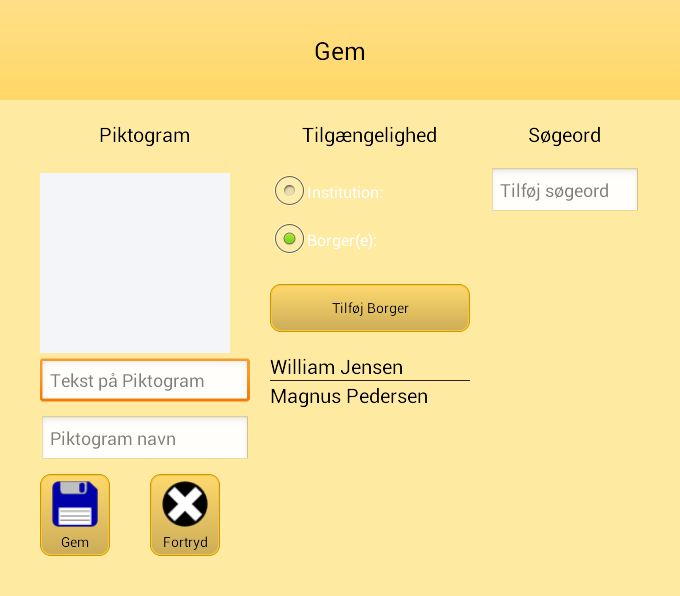
\includegraphics[scale=0.5]{media/sprint4/save_dialog2}
	\caption{The dialogue showing the button where citizens can be given access to a pictogram.}
	\label{fig:save_dialogue2}
\end{figure}

When the button \textit{Tilføj Borger} is clicked a new dialogue will show up where the citizens can be clicked, as seen in \figref{fig:save_dialogue3}, where the darker fields are chosen whereas the light is not.
The dialogue is a component from the \textit{gComponent} library created by the GUI group in the multi-project.
The text colour on the radio buttons are white due to the library, but should have been black as they are not clearly visible.

\begin{figure}[h]
	\centering
	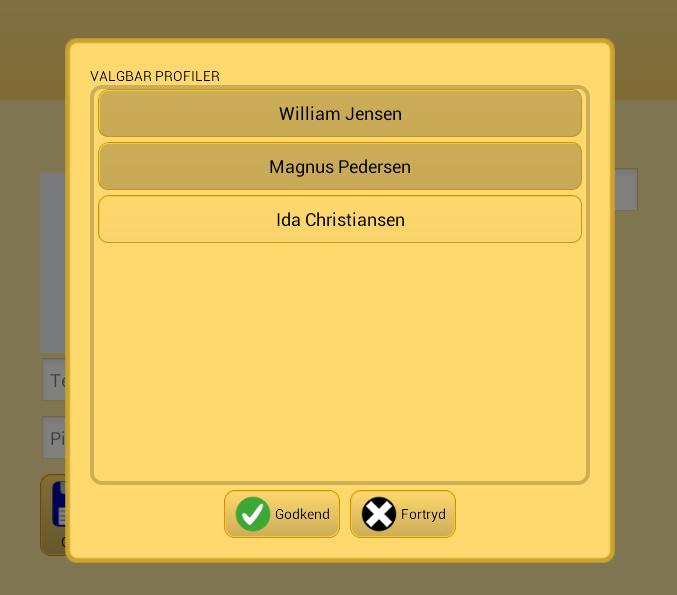
\includegraphics[scale=0.5]{media/sprint4/save_dialog3}
	\caption{The dialogue where citizen are chosen for access.}
	\label{fig:save_dialogue3}
\end{figure}
